
\documentclass{article} % For LaTeX2e
\usepackage{iclr2027_conference,times}

% Optional math commands from https://github.com/goodfeli/dlbook_notation.
\input{math_commands.tex}

\usepackage[utf8]{inputenc}
\usepackage[T1]{fontenc}
\usepackage{hyperref}
\usepackage{url}
\usepackage{booktabs}
\usepackage{array}
\usepackage{amsfonts}
\usepackage{amsmath}
\usepackage{nicefrac}
\usepackage{microtype}
\usepackage{xcolor}
\usepackage{graphicx}
\usepackage{subcaption}
\usepackage{multirow}
\usepackage{enumitem}
\usepackage{placeins}
\usepackage{float}
\usepackage{overpic}


\title{Is There a Platonic Tree? Calibrating Latent Hyperbolicity in Foundation Models}

% Authors must not appear in the submitted version. They should be hidden
% as long as the \iclrfinalcopy macro remains commented out below.
% Non-anonymous submissions will be rejected without review.





% The \author macro works with any number of authors. There are two commands
% used to separate the names and addresses of multiple authors: \And and \AND.
%
% Using \And between authors leaves it to \LaTeX{} to determine where to break
% the lines. Using \AND forces a linebreak at that point. So, if \LaTeX{}
% puts 3 of 4 authors names on the first line, and the last on the second
% line, try using \AND instead of \And before the third author name.

\newcommand{\fix}{\marginpar{FIX}}
\newcommand{\new}{\marginpar{NEW}}

%\iclrfinalcopy % Uncomment for camera-ready version, but NOT for submission.
\begin{document}


\maketitle

\begin{abstract}
Hyperbolic methods for representation learning rest on a premise we call latent hyperbolicity: standard models are already tree-like, because their class geometry scores a low Gromov $\delta$. We show that a low raw reading is what high dimension, an anisotropic spectrum and a maximum over sampled quadruples produce on their own, and we build an instrument that reads every score as an excess over a random cloud of the same shape, ranks it against 200 matched replicates, and adds a depth test whose false-alarm rate and power are measured on real clouds. Across 12 vision backbones, 6 datasets and 16 text models, the premise does not survive: on image features the excess sits within null noise in most cells (model-dataset pairs). Class centroids do carry clustered structure in 49 of 72 cells, but a star already produces it; hierarchy above the superclasses is certified in only 4 of 12 ImageNet backbones, by a test that never fires on randomized hubs, and a backbone trained in hyperbolic space shows the same clustering, no detected depth, and embeddings that never leave the near-flat regime. The trees are moderately shared: the naive comparison manufactures an island, and once the clustering cut is controlled every recipe recovers the human taxonomy partially, with the self-supervised tree living in angles rather than distances. Read correctly, foundation models organize classes into clustered structure that is occasionally hierarchical and moderately shared; they do not converge to one common tree, and their raw tree-likeness is not evidence for hyperbolic geometry.
\end{abstract}




\section{Introduction}
\label{sec:introduction}

Semantic knowledge is hierarchical, and hyperbolic space is the natural geometric home for hierarchies \citep{nickel2017poincare, sarkar2011low, ganea2018hyperbolic, chami2019hyperbolic}. A line of work therefore imposes it on representations at training time, from vision to vision--language and language \citep{Khrulkov_2020_CVPR, ermolov2022hyperbolic, atigh2022hyperbolic, bdeir2024fully, desai2023meru, pal2025compositional, chen2022fully, he2026helm, sinha2024learning}. These methods cite a premise, which we call \emph{latent hyperbolicity}: standard models already organize concepts in a tree-like metric structure. The evidence is a single number, the Gromov $\delta$ of their features: $\delta$ is zero for a metric tree and grows as a metric departs from one, and the measured values are low, on CNN and ViT features \citep{Khrulkov_2020_CVPR, bdeir2024fully}, on token embeddings \citep{yang2025hyperbolic} and on word vectors \citep{tifrea2019poincare}. Those readings are taken at the sample level, on individual images or tokens rather than on classes, and they are never calibrated: a value is called low on its own, without asking what a structureless cloud of the same dimension and spectrum would score. Is the premise right, and what does it license? Figure~\ref{fig:concept} shows why a low reading is not enough: a structureless cloud, a star of clusters without depth and a tree with depth cast the same shadow.

\begin{figure}[H]
\centering
\IfFileExists{figures/fig1_concept.pdf}%
{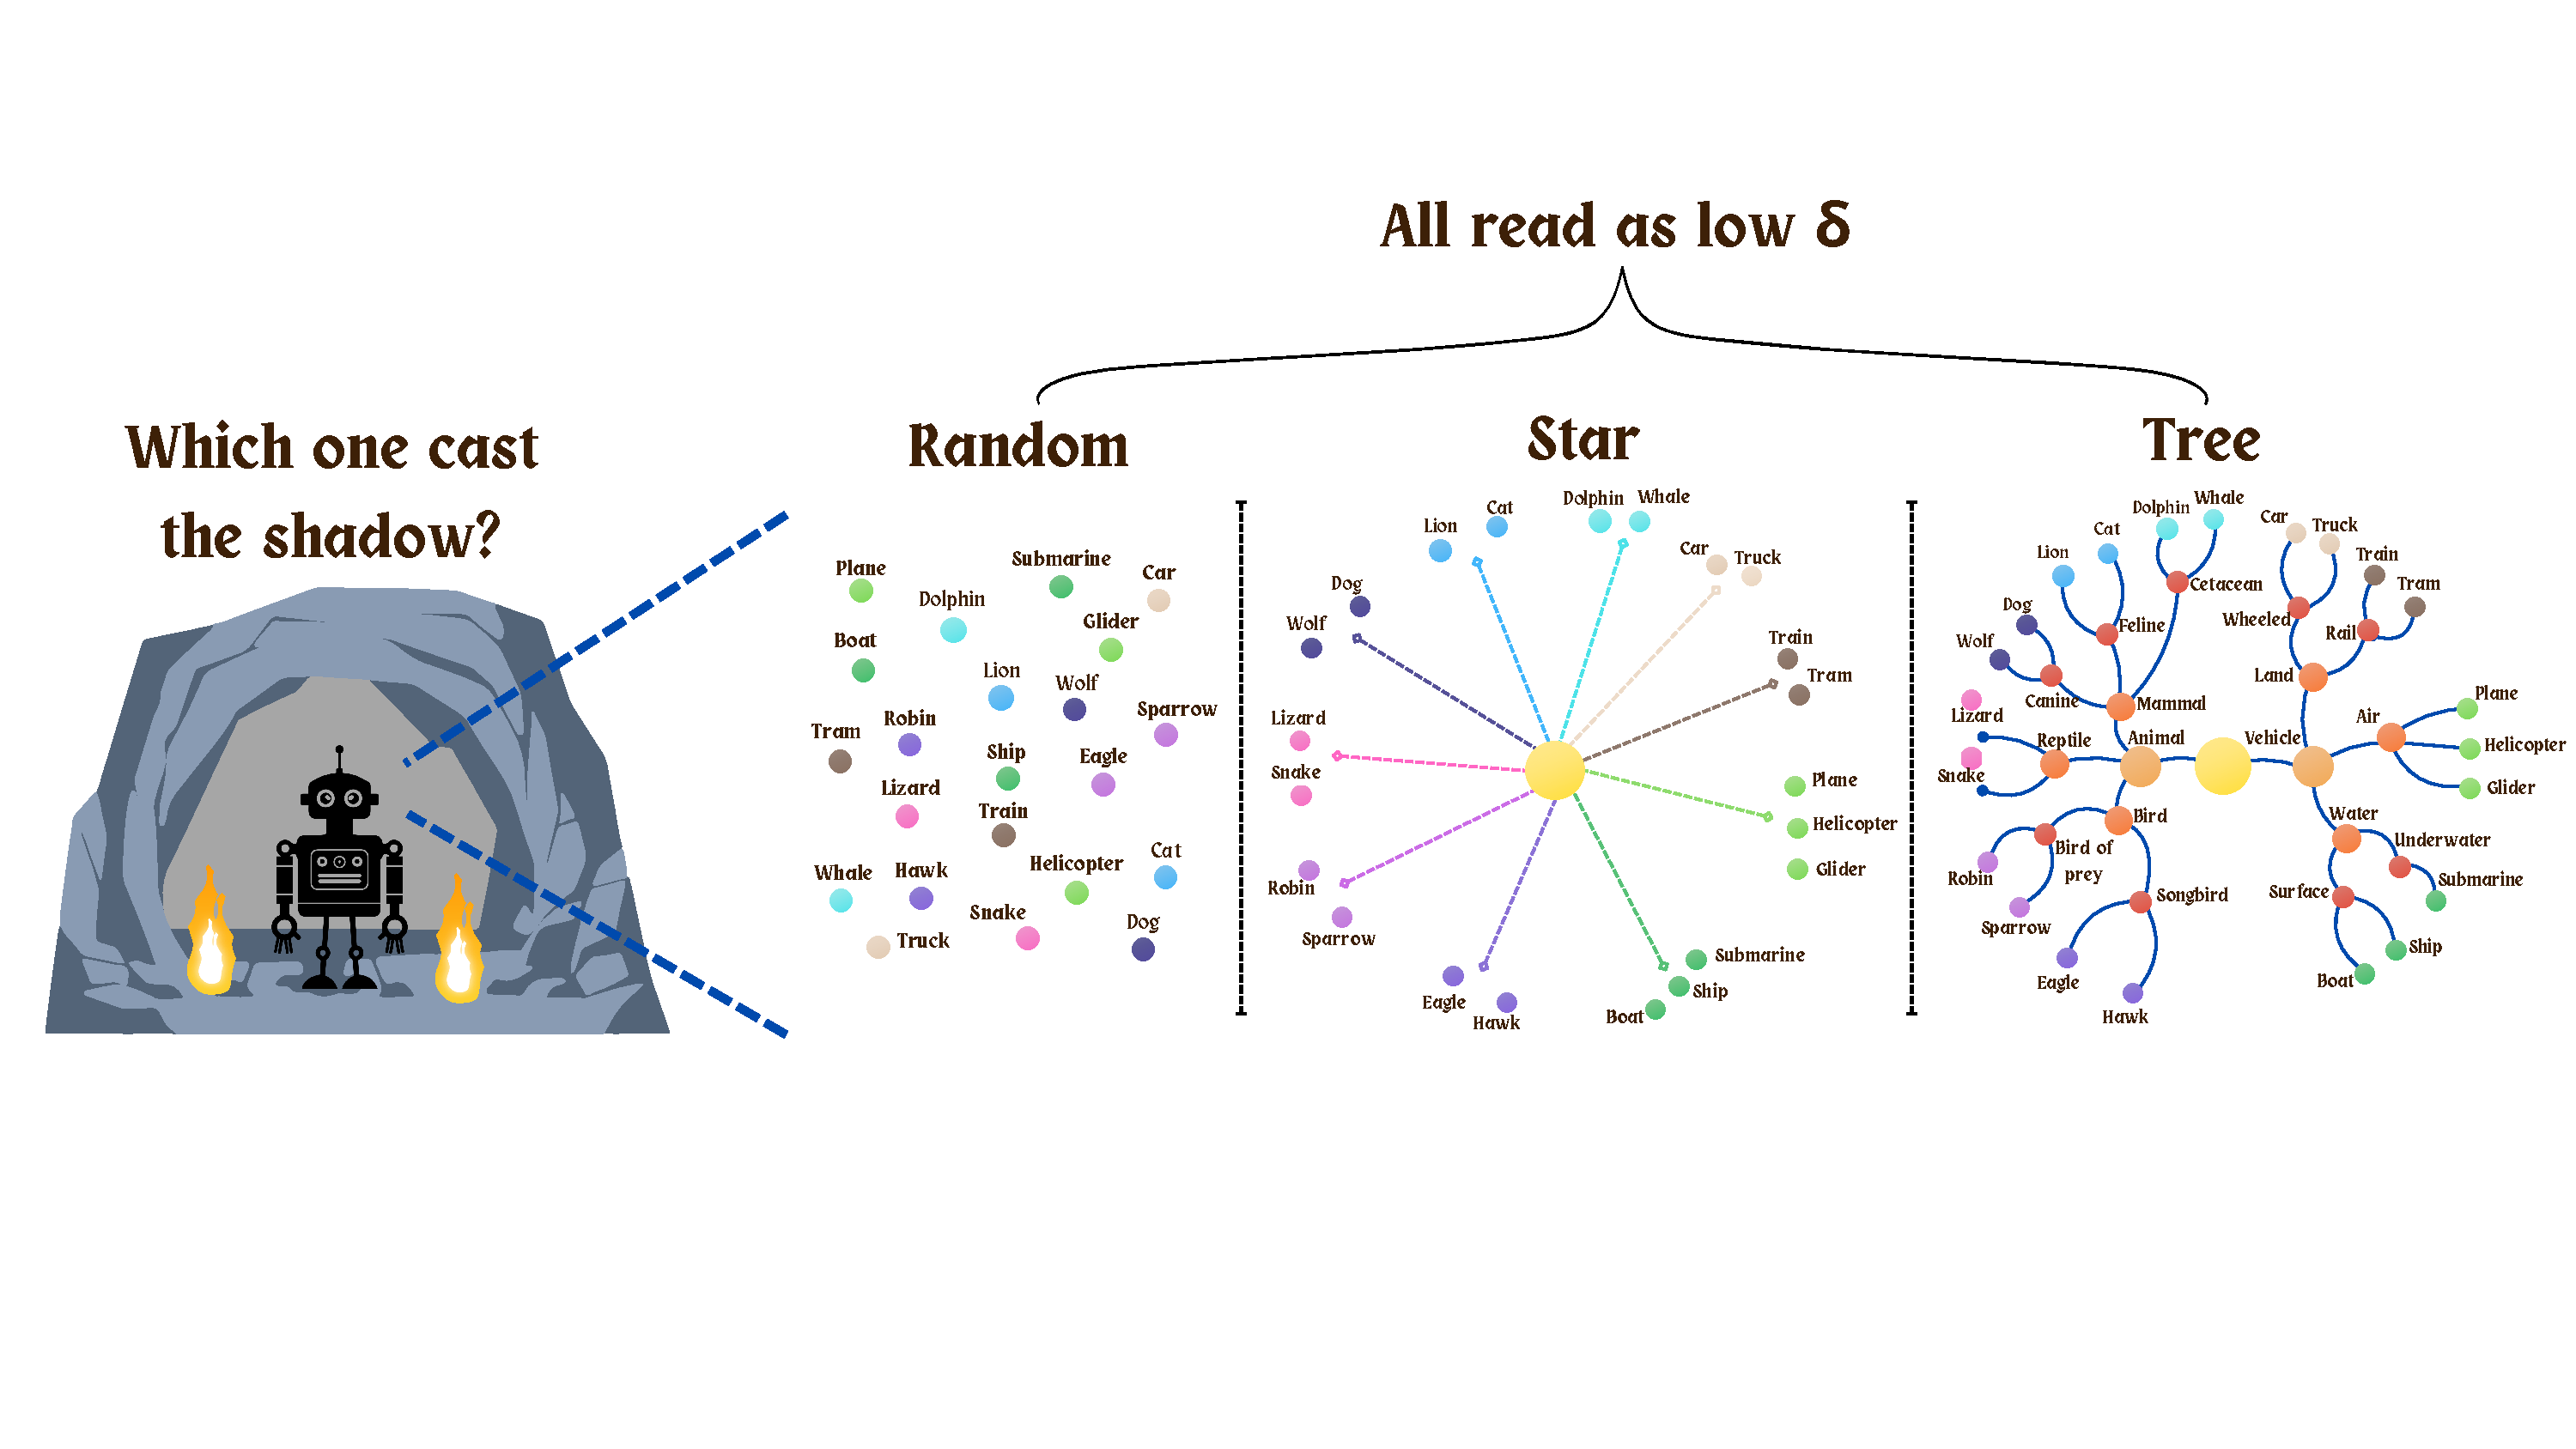
\includegraphics[width=\textwidth, trim=23 229 3 232]{figures/fig1_concept.pdf}}
{\fbox{\parbox[c][1.4in][c]{\dimexpr\textwidth-2\fboxsep-2\fboxrule\relax}{\centering \texttt{figures/fig1\_concept.pdf} (conceptual figure, drawn by the authors; same-size placeholder)}}}
\caption{\textbf{Plato's cave: a random cloud, a star and a tree cast the same shadow.} An observer who sees only shadows cannot tell which object cast them, and a raw $\delta$ is such a shadow: points with no structure, clusters around a hub, and a nested hierarchy all read as low $\delta$. The instrument reads the objects instead of the shadow: no structure beyond the null in the cloud, clusters without depth in the star, clusters with depth in the tree.}
\label{fig:concept}
\end{figure}

Why is the shadow low? Gromov $\delta$ assigns zero to trees \citep{Gromov1987}, but three artifacts push it down without any hierarchy. High-dimensional clouds concentrate toward equidistance \citep{beyer1999nearest, aggarwal2001surprising}, which is a degenerate star tree: we call this the \emph{dimension confound}, the geometric face of the width confounder of \citet{groger2026aristotelian}. Anisotropic spectra mimic low-dimensional behavior: the \emph{spectrum confound}. And the supremum over sampled quadruples is a one-quadruple extreme that does not converge \citep{fournier2015computing}: the \emph{statistic confound}. The three are visible in real models: GPT-2 M sits at its matched null despite a low raw reading, and classic sentence embedders share their raw reading with vision-contrastive models while carrying none of their structure.

We build the instrument that reads $\delta$ correctly. It calibrates the estimator on reference geometries, expresses every reading as an \emph{excess} over a null cloud matched in dimension and covariance spectrum, ranks that excess against matched replicates, and adds a \emph{depth test} whose false-alarm rate and power are measured on real clouds. With it we ask of geometry what convergence work asks of similarity \citep{huh2024platonic, groger2026aristotelian}: what survives calibration, and is it shared? They calibrate similarity across models; we calibrate geometry within a model, and comparing trees across models needs a calibration of its own.

\textbf{The answer has three parts.} On image features the excess sits within null noise in most cells and is a fraction of the null where it survives, so the premise does not survive calibration as stated. On class centroids, clustered structure is genuine in 49 of 72 cells, but a star already produces it. Hierarchy above the superclasses is certified in 4 of 12 ImageNet backbones by a test that never fires on real clouds with randomized hubs, and a backbone trained in hyperbolic space shows the same clustering and no detected depth. The trees are moderately shared: the naive comparison manufactures an island, and once the clustering cut is controlled a moderate gap remains, every recipe recovers the human taxonomy partially, more so with supervision, and the self-supervised structure lives in angles.

\textbf{Our contributions are:}
\begin{enumerate}[topsep=0pt,itemsep=1pt,leftmargin=*]
\item \textbf{The instrument.} Estimator calibration, spectrum-matched nulls read as corrected ranks, and a depth test with measured false-alarm rate and power.
\item \textbf{The census.} Clustered structure in most models, hierarchy certified in a few, and a hyperbolic backbone as the control for imposing the geometry.
\item \textbf{The map of trees.} The island is an artifact of the cut; sharing is graded and supervision-dependent, and the self-supervised tree is angular.
\item \textbf{Consequences for practice.} What to measure before imposing curvature, and which zero-cost readout collects what is there.
\end{enumerate}

\section{Related Work}
\label{sec:related}

Reading $\delta$ against a matched reference has precedent in network science, where the $\delta$ of real graphs is compared with that of random graphs of comparable size \citep{narayan2011curvature, kennedy2013hyperbolicity, adcock2013treelike}; we bring the idea to embedding clouds, where the reference must match dimension and spectrum. The analyses of learned representations characterize Euclidean structure and do not test for tree-likeness: representation similarity, intrinsic dimension and neural collapse \citep{kornblith2019cka, ansuini2019intrinsic, pope2021intrinsic, papyan2020prevalence}. Closest to us is the work on representational convergence: the Platonic Representation Hypothesis \citep{huh2024platonic} argues that models converge toward shared representations, and its cross-modal convergence has been stress-tested at scale \citep{koepke2026cave}; \citet{groger2026aristotelian} show that permutation-calibrated similarity removes most of that convergence while local neighborhood structure survives, and \citet{park2024geometry} read concept hierarchy in language models from the orthogonality of concept directions. We are the geometric complement of this program: the same calibration applied within a model instead of across models, with a depth test measured on real clouds, a hyperbolic backbone as the control for imposing the geometry, and a calibration of the tree-to-tree comparison itself.


\section{The Instrument}
\label{sec:instrument}


If the premise were right, a low raw reading would be evidence on its own. It is not, so this section builds the measurement layer in whose units every later claim is stated: what $\delta$ is, how it is estimated, where it is read, and what it is compared with.

\paragraph{Gromov $\delta$.} Tree-likeness is measured on quadruples. Take any four points $w,x,y,z$ of a metric space with distance $d$. They can be paired in three ways, and each pairing has a sum of two distances:
\begin{equation}
d(w,x)+d(y,z),\qquad d(w,y)+d(x,z),\qquad d(w,z)+d(x,y).
\label{eq:pairings}
\end{equation}
Sort the three sums as $S_{\max}\ge S_{\mathrm{mid}}\ge S_{\min}$. In a tree the two largest sums are always equal, because the two pairings that cross the trunk traverse the same path, so the four-point defect $(S_{\max}-S_{\mathrm{mid}})/2$ is zero; the further a metric is from a tree, the larger the defect can become. Gromov $\delta$ is the worst case, the supremum of the defect over all quadruples \citep{Gromov1987}. A metric tree has $\delta=0$. Euclidean space has no bound at all: enlarging a square enlarges its defect in proportion. Hyperbolic space sits in between, with a bounded defect whose value for the hyperbolic plane is known, $\ln 2$ under this definition \citep{nica2016strong}.

\paragraph{Estimation and normalization.} Three steps turn $\delta$ into a number that can be compared across models. First, a thousand centroids have far more quadruples than can be enumerated, so the defect is computed on half a million random quadruples. Second, the largest defect in that sample is a poor estimate of the supremum: it belongs to a single extreme quadruple and keeps growing as more quadruples are drawn \citep{fournier2015computing}. We therefore read the 99.9th percentile of the sampled defects, $\hat\delta_{99.9}$, the value that 99.9 per cent of them fall below: it keeps the tail of the defects, the intent of the supremum, but it is set by hundreds of quadruples rather than by one. It also does not move with the sample size: across quadruple budgets the ImageNet reading drifts by less than half its own spread (Table~\ref{tab:q8-robust}). Third, the defect grows with the size of the point set, so we divide by the diameter, the largest pairwise distance:
\begin{equation}
\delta_{\text{norm}}=\frac{\hat\delta_{99.9}}{\mathrm{diam}}.
\label{eq:deltanorm}
\end{equation}
On this scale a tree reads zero, and a hyperbolic region of radius four or more reads below a sphere (Table~\ref{tab:q10-calibration}). What a structureless cloud reads on it is the next question.



\begin{figure}[t]
\centering

\includegraphics[width=\linewidth]{figures/fig_overview.pdf}
\caption{\textbf{The raw reading cannot be read on its own.} (a)~Each ImageNet backbone's raw reading (filled) and what a structureless cloud of the same dimension and spectrum reads (hollow); the nulls drift down with the dimension, and the segment between the two is the excess. (b)~Two cells with the same raw reading and opposite verdicts: on ViT-T image features the null sits at the reading, on SigLIP-B centroids far above it.
}
\label{fig:overview}
\end{figure}

\paragraph{The premise lives at the sample level, hierarchy lives at the class level.} The premise is read on the per-image features of frozen models, where the literature measures it. Hierarchy is measured on class centroids: in vision, the mean of each class's cached training embeddings, a hundred per class on ImageNet; in text, the embeddings of ``a photo of a \{class\}'' over the ImageNet classes. A \emph{cell} is one pair of model and class set; the census covers 12 vision backbones on 6 datasets and 16 text models. The raw reading of a cell is $\delta_{\text{norm}}$ of Eq.~\ref{eq:deltanorm}, averaged over ten quadruple seeds; the supremum, the pre-specified statistic, is reported in the appendix for the reason given below.

\paragraph{A low raw reading is not evidence.} Calibrated on reference geometries, the estimator recovers the tree zero and the $\ln 2$ constant of $\mathbb{H}^2$, and spheres stay high. Iid Gaussians, which have no structure at all, drift lower as the dimension grows (Table~\ref{tab:q10-calibration}). Figure~\ref{fig:overview}a shows the same drift on the twelve ImageNet backbones: the null of each moves with its dimension, so the gap, not the level, is the reading. That drift is the dimension confound in its purest form: the raw reading of a real backbone must be compared with the reading of a structureless cloud of the same shape.

\paragraph{The reading is an excess over a matched null.} For every cell we synthesize null clouds with the same $n$, $d$, mean and covariance spectrum. We use the Haar construction throughout: random orthogonal coefficients recombined with the real singular values, so the sample spectrum is exact. In plain terms, the spectrum null is a cloud with the same shape as the real one and no structure inside it; the hub null of Section~\ref{sec:form} keeps every cluster of the real cloud and only rearranges where the clusters sit. The \textbf{excess} is the raw reading minus the mean reading of 200 such replicates. The primary evidence is the \emph{percentile rank}, the number of replicates above the real value, and its left-tail $p$. A cell is \emph{genuine} when its Benjamini--Hochberg-corrected $p$ across the census is at most five per cent; we use the word in this sense only. A negative genuine excess certifies \emph{clustered structure}; the word ``tree-like'' is reserved for the depth test of Section~\ref{sec:form}. A positive excess means less tree-like than chance given the spectrum (Appendix~\ref{app:nulls}). Figure~\ref{fig:overview}b shows two cells with the same raw reading and opposite verdicts.


\paragraph{Projection and tasks.} A parameter-free map centers the features, scales the 95th-percentile norm to radius $1/\sqrt2$ and preserves directions, so Euclidean, Poincar\'{e} and cosine readouts can be compared on the intact representation; nearest-centroid and 5-way 5-shot classification score them for Section~\ref{sec:practice} (Appendix~\ref{app:corollary}). With the instrument in place, we read the premise where it is read.


\section{Findings I: Latent Hyperbolicity, Calibrated}
\label{sec:form}


\begin{figure}[t]
\centering

\includegraphics[width=\linewidth]{figures/fig_excess_panel.pdf}
\caption{\textbf{Clustered structure is the rule at the class level.} Excess of the reading of record over its matched null, one panel per dataset, one marker per backbone; filled markers are genuine cells. Almost every marker sits left of zero, most are filled, the flat datasets scatter around zero, and the DINOv2 rows reach furthest left on CIFAR-10. % expR52_census_haar_p999_200.csv
}
\label{fig:excess}
\end{figure}

\begin{table}[t]
\centering
\scriptsize
\setlength{\tabcolsep}{2.6pt}
\begin{tabular}{l l c c c c c c | c c}
\toprule
 & & \multicolumn{6}{c|}{class level (centroids)} & \multicolumn{2}{c}{sample level (images)} \\ \cmidrule(lr){3-8}\cmidrule(lr){9-10}
model & family & $\hat\delta_{99.9}$ IN & excess IN & $r$/200 ($p$) & exc.\ C100 & exc.\ C10 & $\rho_{\text{WN}}$ & exc.\ C100 & exc.\ DTD \\
\midrule
ViT-T & sup. & $0.088$ & $-0.005^{\circ}$ & 169 (.159) & $-0.006^{\circ}$ & $-0.021^{\circ}$ & $+0.52$ & $-0.002^{\circ}$ & $-0.000^{\circ}$ \\
ViT-S & sup. & $0.063$ & $-0.012$ & 200 (.005) & $-0.000^{\circ}$ & $-0.056$ & $+0.50$ & $+0.005^{\circ}$ & $-0.006$ \\
ViT-B & sup. & $0.054$ & $-0.016$ & 200 (.005) & \textbf{$+0.006^{\circ}$} & $-0.050$ & $+0.49$ & $+0.003^{\circ}$ & $-0.008$ \\
ViT-L & sup. & $0.055$ & $-0.016$ & 200 (.005) & $-0.020$ & $-0.060$ & $+0.53$ & $-0.004^{\circ}$ & $-0.007$ \\
\midrule
DINO-B & SSL & $0.055$ & $-0.020$ & 200 (.005) & $-0.032$ & $-0.061$ & $+0.36$ & $-0.004^{\circ}$ & $+0.001^{\circ}$ \\
DINOv2-S & SSL & $0.053$ & $-0.016$ & 200 (.005) & $-0.031$ & $-0.071$ & $+0.22$ & $-0.005$ & $+0.006^{\circ}$ \\
DINOv2-B & SSL & $0.034$ & $-0.017$ & 200 (.005) & $-0.031$ & $-0.112$ & $+0.18$ & $-0.009$ & $-0.002^{\circ}$ \\
DINOv2-L & SSL & $0.030$ & $-0.014$ & 200 (.005) & $-0.035$ & $-0.128$ & $+0.18$ & $-0.013$ & $-0.006$ \\
DINOv2-G & SSL & $0.033$ & $-0.008$ & 200 (.005) & $-0.040$ & $-0.130$ & $+0.20$ & $-0.023$ & $-0.008$ \\
\midrule
CLIP-B & contr. & $0.084$ & $-0.007^{\circ}$ & 172 (.144) & $-0.019$ & $-0.036$ & $+0.57$ & $-0.006^{\circ}$ & $+0.002^{\circ}$ \\
CLIP-L & contr. & $0.076$ & $-0.009$ & 197 (.020) & $-0.018$ & $-0.043$ & $+0.59$ & $+0.004^{\circ}$ & $-0.001^{\circ}$ \\
SigLIP-B & contr. & $0.075$ & $-0.008^{\circ}$ & 189 (.060) & $-0.022$ & $-0.050$ & $+0.58$ & $-0.007$ & $-0.004^{\circ}$ \\
\bottomrule
\end{tabular}
\caption{\textbf{Clustered structure is the rule at the class level; the sample-level reading sits within null noise in most cells.} One row per backbone. $\hat\delta_{99.9}$: raw ImageNet reading; excess: $\hat\delta_{99.9}$ minus the mean of 200 Haar spectrum-matched null replicates; $r$/200: replicates above the real value, with the left-tail $p=(1+\#\{\text{null}\le\text{real}\})/201$; genuine: Benjamini--Hochberg-corrected $p\le0.05$ over the 72 cells; $^{\circ}$: not genuine; bold: less clustered than the null. $\rho_{\text{WN}}$: Spearman correlation of inter-centroid and WordNet distances. Sample level: the same reading on $\approx$1000 stratified training images per cell, BH over those 24 cells: genuine in 10 of 24 (full table in Appendix~\ref{app:sample}). With centroid-resampling and estimator noise folded into the null, or the census repeated on 30 resampled centroid sets, the genuine count is 42--47 of 72 (Table~\ref{tab:b38-joint}). Cross-dataset magnitudes are not comparable. The other datasets, the supremum reading and the task columns are in Table~\ref{tab:census-extra}; all four null$\times$statistic verdicts per cell in Table~\ref{tab:b21-2x2}. % expR52_census_haar_p999_200.csv, exp3_alignment.csv, expR62_samplelevel_record.csv, expR66_joint_sensitivity_summary.csv
}
\label{tab:census}
\end{table}


If standard models were latently hyperbolic, the instrument should find an excess on their image features, where the premise is read. It finds one within null noise in most cells, and what survives lives on class centroids, where a star already passes the census.

\paragraph{The premise does not survive calibration.} We read it first on per-image features, roughly a thousand stratified training images per cell for CIFAR-100 and DTD, where the raw reading lies in the low band the literature reports. Calibrated, it is not genuine in most cells, and where it is genuine it removes between 7 and 39 per cent of the null reading, the larger figure for DINOv2-G on CIFAR-100 images, and it is largest in the DINOv2 family, whose structure is the angular tree of Section~\ref{sec:content}, which cosine collects. This is the reading that motivates hyperbolic methods, and calibrated it is what a random cloud of the same dimension and spectrum produces, up to a fraction of the null (Table~\ref{tab:q3-sample}).

\paragraph{Clustered structure is the rule.} Table~\ref{tab:census} gives the census of record. Figure~\ref{fig:excess} shows it: almost every marker sits left of zero, most are filled, the flat datasets scatter around it, and the DINOv2 rows reach furthest left on CIFAR-10. In 49 of the 72 cells the gap is one that chance does not produce. On ImageNet and CIFAR-100, the two sets with a real hierarchy, the count is 18 of 24. The structure belongs to no single family or architecture: every family contributes genuine cells and two self-supervised ResNets read the same as the ViTs. What moves the reading is the label set: the smallest backbone is genuine on one dataset only, the flat datasets sit at the resolution limit of ten classes, and a class-count control shows that the reading follows the hierarchy of the labels rather than their number (Table~\ref{tab:q8-robust}). % expR52_census_haar_p999_200.csv, expR59_imagenet_bootstrap_summary.csv, expR45_convnet_rows.csv, expR60_c_sweep_record.csv


\bibliography{iclr2027_conference}
\bibliographystyle{iclr2027_conference}

\appendix
\section{Appendix}
You may include other additional sections here.


\end{document}
